\section{Kevin Stuka}
\label{sec:Kevin_Stuka}
\subsection{Fotografia QUEBONAFIDE}
\begin{figure}[h]
    \centering
    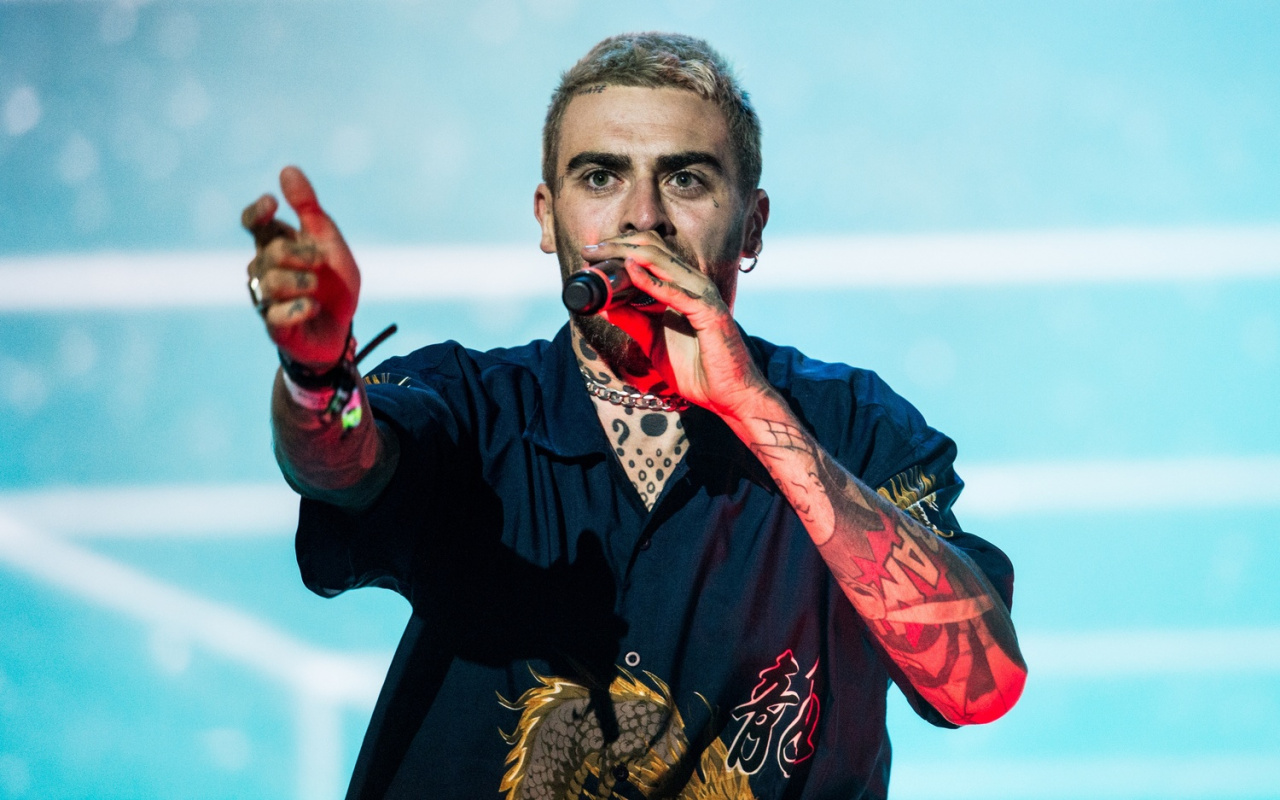
\includegraphics[scale = 0.35]{pictures/quebo.png}
    \caption{Idol}
    \label{fig:quebo}
\end{figure}
\subsection{Dane ze sprzedaży}
\begin{tabular}{|l|l|l|}
\hline
Nazwa albumu    & Uzyskany certyfikat & Ilość sprzedanych sztuk fizycznych \\ \hline
Ezoteryka       & Platynowa płyta     & 30 tys+                            \\ \hline
Egzotyka        & Diamentowa płyta    & 150 tys+                           \\ \hline
Soma 0.5 mg     & Diamentowa płyta    & 150 tys+                           \\ \hline
Romantic Psycho & Diamentowa płyta    & 150tys+                            \\ \hline
\end{tabular}

\subsection{Dyskografia}
Pozostałe minialbumy/mixtape'y:
\begin{itemize}
    \item Hip-Hop 2.0
    \item Demówka EP
    \item Dla fanów eklektyki EP/Dla fanek euforii EP
    \item No to bajka Ep
    \item Płyta roku
    \item Eklektyka
    \item Erotyka
    \item Elektryka
    \item 0.25 mg
\end{itemize}
Fav kawałki:
\begin{enumerate}
    \item Refrentrochęjaklanadelrey
    \item Niepłaczeponotredam
    \item Ciernie
\end{enumerate}
\subsection{Biografia}
\textbf{Quebonafide}, a właściwie Kuba Grabowski, jest polskim raperem i autorem tekstów. Urodził się 7 lipca 1991 roku w Ciechanowie. Pseudonim rapera jest połączeniem fraz Quebo, czyli imienia rapera, oraz pochodzącego z łaciny \emph{bona fides}, które oznacza \emph{działający w dobrej wierze}. Quebo znany jest ze swojego nietuzinkowego wizerunku, w tym kolorowych włosów i wszechobecnych tatuaży (posiada nawet tatuaż na wewnętrznej stronie dolnej wargi). Swoje pierwsze kroki na rynku muzycznym raper stawiał już w 2008 roku, jednak nie przyniosły mu oczekiwanego rozgłosu. Przełomowym momentem na samym początku muzycznej działalności Quebonafide była premiera jego mixtapu zatytułowanego Eklektyka. Stopniowo zaczął zdobywać rozpoznawalność w polskim środowisku hip-hopowym. W 2014 roku Quebo założył wytwórnię QueQuality. Rok później wydał swoją pierwszą płytę studyjną zatytułowaną Ezoteryka, która z czasem uzyskała status płyty platynowej, a jej twórca ruszył w pierwszą trasę koncertową o nazwie Ezoteryka Tour. Raper szybko poszerzał rzesze swoich fanów spragnionych hip-hopowej świeżości na polskim rynku muzycznym. Nie spoczął jednak na manowcach i już w 2017 roku ukazała się kolejna płyta artysty zatytułowana Egzotyka. \underline{Egzotyka stała się najlepiej sprzedającą płytą w Polsce w 2017 roku}, a jej twórca jednym z najpopularniejszych i najbardziej docenianych twórców. Prawdziwą sensację przyniosła jednak współpraca z innym raperem, \textbf{Taco Hemingwayem}. Wspólnie nagrali płytę Soma 0,5 mg i ruszyli w promującą ją trasę koncertową. Najbardziej znany utwór z tego albumu, Tamagotchi, przez długi czas zajmował pierwsze miejsca wielu polskich list przebojów oraz stał się hitem mediów społecznościowych. W 2020 roku premierę miał czwarty krążek artysty zatytułowany Romantic Psycho. Jego popularność stale rośnie i odzwierciedla się w ilości fanów. Quebo jest bowiem pierwszym raperem w Polsce z milionem obserwujących na Instagramie. W ostatnich latach generuje olbrzymie zainteresowanie, co przejawia się choćby tym, że pięć jego płyt zajmuje miejsca w pierwszej szóstce oficjalnej listy najlepiej sprzedających się płyt w Polsce. Był pięciokrotnie nominowany do nagrody Fryderyków, w tym raz otrzymał nagrodę w kategorii „Album roku hip-hop” za płytę Soma 0,5 mg. Dwa razy nominowany był do nagrody Bestsellerów Empiku w kategorii „Muzyka polska ” za albumy Soma 0,5 mg oraz Egzotyka.
\subsection{Granice}
Czy dla Quebo istnieją jakieś granice? Odpowiedź poprzez wzór: 
\[lim_{n\to\infty}-1^n\]
NIE!
